% Options for packages loaded elsewhere
% Options for packages loaded elsewhere
\PassOptionsToPackage{unicode}{hyperref}
\PassOptionsToPackage{hyphens}{url}
\PassOptionsToPackage{dvipsnames,svgnames,x11names}{xcolor}
%
\documentclass[
]{article}
\usepackage{xcolor}
\usepackage[margin=1in]{geometry}
\usepackage{amsmath,amssymb}
\setcounter{secnumdepth}{-\maxdimen} % remove section numbering
\usepackage{iftex}
\ifPDFTeX
  \usepackage[T1]{fontenc}
  \usepackage[utf8]{inputenc}
  \usepackage{textcomp} % provide euro and other symbols
\else % if luatex or xetex
  \usepackage{unicode-math} % this also loads fontspec
  \defaultfontfeatures{Scale=MatchLowercase}
  \defaultfontfeatures[\rmfamily]{Ligatures=TeX,Scale=1}
\fi
\usepackage{lmodern}
\ifPDFTeX\else
  % xetex/luatex font selection
\fi
% Use upquote if available, for straight quotes in verbatim environments
\IfFileExists{upquote.sty}{\usepackage{upquote}}{}
\IfFileExists{microtype.sty}{% use microtype if available
  \usepackage[]{microtype}
  \UseMicrotypeSet[protrusion]{basicmath} % disable protrusion for tt fonts
}{}
\makeatletter
\@ifundefined{KOMAClassName}{% if non-KOMA class
  \IfFileExists{parskip.sty}{%
    \usepackage{parskip}
  }{% else
    \setlength{\parindent}{0pt}
    \setlength{\parskip}{6pt plus 2pt minus 1pt}}
}{% if KOMA class
  \KOMAoptions{parskip=half}}
\makeatother
% Make \paragraph and \subparagraph free-standing
\makeatletter
\ifx\paragraph\undefined\else
  \let\oldparagraph\paragraph
  \renewcommand{\paragraph}{
    \@ifstar
      \xxxParagraphStar
      \xxxParagraphNoStar
  }
  \newcommand{\xxxParagraphStar}[1]{\oldparagraph*{#1}\mbox{}}
  \newcommand{\xxxParagraphNoStar}[1]{\oldparagraph{#1}\mbox{}}
\fi
\ifx\subparagraph\undefined\else
  \let\oldsubparagraph\subparagraph
  \renewcommand{\subparagraph}{
    \@ifstar
      \xxxSubParagraphStar
      \xxxSubParagraphNoStar
  }
  \newcommand{\xxxSubParagraphStar}[1]{\oldsubparagraph*{#1}\mbox{}}
  \newcommand{\xxxSubParagraphNoStar}[1]{\oldsubparagraph{#1}\mbox{}}
\fi
\makeatother

\usepackage{color}
\usepackage{fancyvrb}
\newcommand{\VerbBar}{|}
\newcommand{\VERB}{\Verb[commandchars=\\\{\}]}
\DefineVerbatimEnvironment{Highlighting}{Verbatim}{commandchars=\\\{\}}
% Add ',fontsize=\small' for more characters per line
\usepackage{framed}
\definecolor{shadecolor}{RGB}{241,243,245}
\newenvironment{Shaded}{\begin{snugshade}}{\end{snugshade}}
\newcommand{\AlertTok}[1]{\textcolor[rgb]{0.68,0.00,0.00}{#1}}
\newcommand{\AnnotationTok}[1]{\textcolor[rgb]{0.37,0.37,0.37}{#1}}
\newcommand{\AttributeTok}[1]{\textcolor[rgb]{0.40,0.45,0.13}{#1}}
\newcommand{\BaseNTok}[1]{\textcolor[rgb]{0.68,0.00,0.00}{#1}}
\newcommand{\BuiltInTok}[1]{\textcolor[rgb]{0.00,0.23,0.31}{#1}}
\newcommand{\CharTok}[1]{\textcolor[rgb]{0.13,0.47,0.30}{#1}}
\newcommand{\CommentTok}[1]{\textcolor[rgb]{0.37,0.37,0.37}{#1}}
\newcommand{\CommentVarTok}[1]{\textcolor[rgb]{0.37,0.37,0.37}{\textit{#1}}}
\newcommand{\ConstantTok}[1]{\textcolor[rgb]{0.56,0.35,0.01}{#1}}
\newcommand{\ControlFlowTok}[1]{\textcolor[rgb]{0.00,0.23,0.31}{\textbf{#1}}}
\newcommand{\DataTypeTok}[1]{\textcolor[rgb]{0.68,0.00,0.00}{#1}}
\newcommand{\DecValTok}[1]{\textcolor[rgb]{0.68,0.00,0.00}{#1}}
\newcommand{\DocumentationTok}[1]{\textcolor[rgb]{0.37,0.37,0.37}{\textit{#1}}}
\newcommand{\ErrorTok}[1]{\textcolor[rgb]{0.68,0.00,0.00}{#1}}
\newcommand{\ExtensionTok}[1]{\textcolor[rgb]{0.00,0.23,0.31}{#1}}
\newcommand{\FloatTok}[1]{\textcolor[rgb]{0.68,0.00,0.00}{#1}}
\newcommand{\FunctionTok}[1]{\textcolor[rgb]{0.28,0.35,0.67}{#1}}
\newcommand{\ImportTok}[1]{\textcolor[rgb]{0.00,0.46,0.62}{#1}}
\newcommand{\InformationTok}[1]{\textcolor[rgb]{0.37,0.37,0.37}{#1}}
\newcommand{\KeywordTok}[1]{\textcolor[rgb]{0.00,0.23,0.31}{\textbf{#1}}}
\newcommand{\NormalTok}[1]{\textcolor[rgb]{0.00,0.23,0.31}{#1}}
\newcommand{\OperatorTok}[1]{\textcolor[rgb]{0.37,0.37,0.37}{#1}}
\newcommand{\OtherTok}[1]{\textcolor[rgb]{0.00,0.23,0.31}{#1}}
\newcommand{\PreprocessorTok}[1]{\textcolor[rgb]{0.68,0.00,0.00}{#1}}
\newcommand{\RegionMarkerTok}[1]{\textcolor[rgb]{0.00,0.23,0.31}{#1}}
\newcommand{\SpecialCharTok}[1]{\textcolor[rgb]{0.37,0.37,0.37}{#1}}
\newcommand{\SpecialStringTok}[1]{\textcolor[rgb]{0.13,0.47,0.30}{#1}}
\newcommand{\StringTok}[1]{\textcolor[rgb]{0.13,0.47,0.30}{#1}}
\newcommand{\VariableTok}[1]{\textcolor[rgb]{0.07,0.07,0.07}{#1}}
\newcommand{\VerbatimStringTok}[1]{\textcolor[rgb]{0.13,0.47,0.30}{#1}}
\newcommand{\WarningTok}[1]{\textcolor[rgb]{0.37,0.37,0.37}{\textit{#1}}}

\usepackage{longtable,booktabs,array}
\usepackage{calc} % for calculating minipage widths
% Correct order of tables after \paragraph or \subparagraph
\usepackage{etoolbox}
\makeatletter
\patchcmd\longtable{\par}{\if@noskipsec\mbox{}\fi\par}{}{}
\makeatother
% Allow footnotes in longtable head/foot
\IfFileExists{footnotehyper.sty}{\usepackage{footnotehyper}}{\usepackage{footnote}}
\makesavenoteenv{longtable}
\usepackage{graphicx}
\makeatletter
\newsavebox\pandoc@box
\newcommand*\pandocbounded[1]{% scales image to fit in text height/width
  \sbox\pandoc@box{#1}%
  \Gscale@div\@tempa{\textheight}{\dimexpr\ht\pandoc@box+\dp\pandoc@box\relax}%
  \Gscale@div\@tempb{\linewidth}{\wd\pandoc@box}%
  \ifdim\@tempb\p@<\@tempa\p@\let\@tempa\@tempb\fi% select the smaller of both
  \ifdim\@tempa\p@<\p@\scalebox{\@tempa}{\usebox\pandoc@box}%
  \else\usebox{\pandoc@box}%
  \fi%
}
% Set default figure placement to htbp
\def\fps@figure{htbp}
\makeatother





\setlength{\emergencystretch}{3em} % prevent overfull lines

\providecommand{\tightlist}{%
  \setlength{\itemsep}{0pt}\setlength{\parskip}{0pt}}



 


\makeatletter
\@ifpackageloaded{caption}{}{\usepackage{caption}}
\AtBeginDocument{%
\ifdefined\contentsname
  \renewcommand*\contentsname{Table of contents}
\else
  \newcommand\contentsname{Table of contents}
\fi
\ifdefined\listfigurename
  \renewcommand*\listfigurename{List of Figures}
\else
  \newcommand\listfigurename{List of Figures}
\fi
\ifdefined\listtablename
  \renewcommand*\listtablename{List of Tables}
\else
  \newcommand\listtablename{List of Tables}
\fi
\ifdefined\figurename
  \renewcommand*\figurename{Figure}
\else
  \newcommand\figurename{Figure}
\fi
\ifdefined\tablename
  \renewcommand*\tablename{Table}
\else
  \newcommand\tablename{Table}
\fi
}
\@ifpackageloaded{float}{}{\usepackage{float}}
\floatstyle{ruled}
\@ifundefined{c@chapter}{\newfloat{codelisting}{h}{lop}}{\newfloat{codelisting}{h}{lop}[chapter]}
\floatname{codelisting}{Listing}
\newcommand*\listoflistings{\listof{codelisting}{List of Listings}}
\makeatother
\makeatletter
\makeatother
\makeatletter
\@ifpackageloaded{caption}{}{\usepackage{caption}}
\@ifpackageloaded{subcaption}{}{\usepackage{subcaption}}
\makeatother
\usepackage{bookmark}
\IfFileExists{xurl.sty}{\usepackage{xurl}}{} % add URL line breaks if available
\urlstyle{same}
\hypersetup{
  pdftitle={Primer proyecto en Quarto},
  pdfauthor={Juan Brito},
  colorlinks=true,
  linkcolor={blue},
  filecolor={Maroon},
  citecolor={blue},
  urlcolor={blue},
  pdfcreator={LaTeX via pandoc}}


\title{Primer proyecto en Quarto}
\usepackage{etoolbox}
\makeatletter
\providecommand{\subtitle}[1]{% add subtitle to \maketitle
  \apptocmd{\@title}{\par {\large #1 \par}}{}{}
}
\makeatother
\subtitle{Análisis y Modelado de Datos}
\author{Juan Brito}
\date{2025-10-04}
\begin{document}
\maketitle


\section{Introducción}\label{introducciuxf3n}

Este documento presenta un análisis completo de machine learning
utilizando Quarto para la documentación y visualización de resultados.

\subsection{Objetivos}\label{objetivos}

\begin{itemize}
\tightlist
\item
  Explorar y analizar un conjunto de datos
\item
  Implementar diferentes algoritmos de machine learning
\item
  Comparar el rendimiento de los modelos
\item
  Visualizar los resultados de manera clara
\end{itemize}

\section{Configuración del Entorno}\label{configuraciuxf3n-del-entorno}

\phantomsection\label{setup}
\begin{Shaded}
\begin{Highlighting}[]
\ImportTok{import}\NormalTok{ pandas }\ImportTok{as}\NormalTok{ pd}
\ImportTok{import}\NormalTok{ numpy }\ImportTok{as}\NormalTok{ np}
\ImportTok{import}\NormalTok{ matplotlib.pyplot }\ImportTok{as}\NormalTok{ plt}
\ImportTok{import}\NormalTok{ seaborn }\ImportTok{as}\NormalTok{ sns}
\ImportTok{from}\NormalTok{ sklearn.model\_selection }\ImportTok{import}\NormalTok{ train\_test\_split}
\ImportTok{from}\NormalTok{ sklearn.ensemble }\ImportTok{import}\NormalTok{ RandomForestClassifier}
\ImportTok{from}\NormalTok{ sklearn.linear\_model }\ImportTok{import}\NormalTok{ LogisticRegression}
\ImportTok{from}\NormalTok{ sklearn.metrics }\ImportTok{import}\NormalTok{ classification\_report, confusion\_matrix}
\ImportTok{import}\NormalTok{ warnings}
\NormalTok{warnings.filterwarnings(}\StringTok{\textquotesingle{}ignore\textquotesingle{}}\NormalTok{)}

\CommentTok{\# Configuración de matplotlib}
\NormalTok{plt.style.use(}\StringTok{\textquotesingle{}seaborn{-}v0\_8\textquotesingle{}}\NormalTok{)}
\NormalTok{sns.set\_palette(}\StringTok{"husl"}\NormalTok{)}
\end{Highlighting}
\end{Shaded}

\section{Carga y Exploración de
Datos}\label{carga-y-exploraciuxf3n-de-datos}

\begin{Shaded}
\begin{Highlighting}[]
\CommentTok{\# Ejemplo con datos sintéticos}
\NormalTok{np.random.seed(}\DecValTok{42}\NormalTok{)}
\NormalTok{n\_samples }\OperatorTok{=} \DecValTok{1000}

\CommentTok{\# Generar datos de ejemplo}
\NormalTok{data }\OperatorTok{=}\NormalTok{ \{}
    \StringTok{\textquotesingle{}feature\_1\textquotesingle{}}\NormalTok{: np.random.normal(}\DecValTok{0}\NormalTok{, }\DecValTok{1}\NormalTok{, n\_samples),}
    \StringTok{\textquotesingle{}feature\_2\textquotesingle{}}\NormalTok{: np.random.normal(}\DecValTok{0}\NormalTok{, }\DecValTok{1}\NormalTok{, n\_samples),}
    \StringTok{\textquotesingle{}feature\_3\textquotesingle{}}\NormalTok{: np.random.normal(}\DecValTok{0}\NormalTok{, }\DecValTok{1}\NormalTok{, n\_samples),}
    \StringTok{\textquotesingle{}target\textquotesingle{}}\NormalTok{: np.random.choice([}\DecValTok{0}\NormalTok{, }\DecValTok{1}\NormalTok{], n\_samples, p}\OperatorTok{=}\NormalTok{[}\FloatTok{0.6}\NormalTok{, }\FloatTok{0.4}\NormalTok{])}
\NormalTok{\}}

\NormalTok{df }\OperatorTok{=}\NormalTok{ pd.DataFrame(data)}
\BuiltInTok{print}\NormalTok{(}\SpecialStringTok{f"Forma del dataset: }\SpecialCharTok{\{}\NormalTok{df}\SpecialCharTok{.}\NormalTok{shape}\SpecialCharTok{\}}\SpecialStringTok{"}\NormalTok{)}
\BuiltInTok{print}\NormalTok{(}\SpecialStringTok{f"}\CharTok{\textbackslash{}n}\SpecialStringTok{Primeras 5 filas:"}\NormalTok{)}
\NormalTok{df.head()}
\end{Highlighting}
\end{Shaded}

\begin{verbatim}
Forma del dataset: (1000, 4)

Primeras 5 filas:
\end{verbatim}

\phantomsection\label{load-data}
\begin{tabular}{lrrrr}
\toprule
{} &  feature\_1 &  feature\_2 &  feature\_3 &  target \\
\midrule
0 &   0.496714 &   1.399355 &  -0.675178 &       1 \\
1 &  -0.138264 &   0.924634 &  -0.144519 &       1 \\
2 &   0.647689 &   0.059630 &  -0.792420 &       0 \\
3 &   1.523030 &  -0.646937 &  -0.307962 &       1 \\
4 &  -0.234153 &   0.698223 &  -1.893615 &       0 \\
\bottomrule
\end{tabular}

\subsection{Estadísticas
Descriptivas}\label{estaduxedsticas-descriptivas}

\begin{Shaded}
\begin{Highlighting}[]
\CommentTok{\# Estadísticas descriptivas}
\BuiltInTok{print}\NormalTok{(}\StringTok{"Estadísticas descriptivas:"}\NormalTok{)}
\NormalTok{df.describe()}
\end{Highlighting}
\end{Shaded}

\begin{verbatim}
Estadísticas descriptivas:
\end{verbatim}

\phantomsection\label{describe-data}
\begin{tabular}{lrrrr}
\toprule
{} &    feature\_1 &    feature\_2 &    feature\_3 &       target \\
\midrule
count &  1000.000000 &  1000.000000 &  1000.000000 &  1000.000000 \\
mean  &     0.019332 &     0.070836 &     0.005834 &     0.379000 \\
std   &     0.979216 &     0.997454 &     0.983454 &     0.485381 \\
min   &    -3.241267 &    -2.940389 &    -3.019512 &     0.000000 \\
25\%   &    -0.647590 &    -0.606242 &    -0.648000 &     0.000000 \\
50\%   &     0.025301 &     0.063077 &    -0.000251 &     0.000000 \\
75\%   &     0.647944 &     0.728882 &     0.660915 &     1.000000 \\
max   &     3.852731 &     3.193108 &     3.926238 &     1.000000 \\
\bottomrule
\end{tabular}

\subsection{Visualización de los
Datos}\label{visualizaciuxf3n-de-los-datos}

\begin{Shaded}
\begin{Highlighting}[]
\CommentTok{\# Crear subplots}
\NormalTok{fig, axes }\OperatorTok{=}\NormalTok{ plt.subplots(}\DecValTok{2}\NormalTok{, }\DecValTok{2}\NormalTok{, figsize}\OperatorTok{=}\NormalTok{(}\DecValTok{12}\NormalTok{, }\DecValTok{10}\NormalTok{))}

\CommentTok{\# Histograma de feature\_1}
\NormalTok{axes[}\DecValTok{0}\NormalTok{, }\DecValTok{0}\NormalTok{].hist(df[}\StringTok{\textquotesingle{}feature\_1\textquotesingle{}}\NormalTok{], bins}\OperatorTok{=}\DecValTok{30}\NormalTok{, alpha}\OperatorTok{=}\FloatTok{0.7}\NormalTok{, color}\OperatorTok{=}\StringTok{\textquotesingle{}skyblue\textquotesingle{}}\NormalTok{)}
\NormalTok{axes[}\DecValTok{0}\NormalTok{, }\DecValTok{0}\NormalTok{].set\_title(}\StringTok{\textquotesingle{}Distribución de Feature 1\textquotesingle{}}\NormalTok{)}
\NormalTok{axes[}\DecValTok{0}\NormalTok{, }\DecValTok{0}\NormalTok{].set\_xlabel(}\StringTok{\textquotesingle{}Valor\textquotesingle{}}\NormalTok{)}
\NormalTok{axes[}\DecValTok{0}\NormalTok{, }\DecValTok{0}\NormalTok{].set\_ylabel(}\StringTok{\textquotesingle{}Frecuencia\textquotesingle{}}\NormalTok{)}

\CommentTok{\# Scatter plot feature\_1 vs feature\_2}
\NormalTok{scatter }\OperatorTok{=}\NormalTok{ axes[}\DecValTok{0}\NormalTok{, }\DecValTok{1}\NormalTok{].scatter(df[}\StringTok{\textquotesingle{}feature\_1\textquotesingle{}}\NormalTok{], df[}\StringTok{\textquotesingle{}feature\_2\textquotesingle{}}\NormalTok{], }
\NormalTok{                           c}\OperatorTok{=}\NormalTok{df[}\StringTok{\textquotesingle{}target\textquotesingle{}}\NormalTok{], cmap}\OperatorTok{=}\StringTok{\textquotesingle{}viridis\textquotesingle{}}\NormalTok{, alpha}\OperatorTok{=}\FloatTok{0.6}\NormalTok{)}
\NormalTok{axes[}\DecValTok{0}\NormalTok{, }\DecValTok{1}\NormalTok{].set\_title(}\StringTok{\textquotesingle{}Feature 1 vs Feature 2\textquotesingle{}}\NormalTok{)}
\NormalTok{axes[}\DecValTok{0}\NormalTok{, }\DecValTok{1}\NormalTok{].set\_xlabel(}\StringTok{\textquotesingle{}Feature 1\textquotesingle{}}\NormalTok{)}
\NormalTok{axes[}\DecValTok{0}\NormalTok{, }\DecValTok{1}\NormalTok{].set\_ylabel(}\StringTok{\textquotesingle{}Feature 2\textquotesingle{}}\NormalTok{)}
\NormalTok{plt.colorbar(scatter, ax}\OperatorTok{=}\NormalTok{axes[}\DecValTok{0}\NormalTok{, }\DecValTok{1}\NormalTok{])}

\CommentTok{\# Box plot por target}
\NormalTok{df.boxplot(column}\OperatorTok{=}\StringTok{\textquotesingle{}feature\_1\textquotesingle{}}\NormalTok{, by}\OperatorTok{=}\StringTok{\textquotesingle{}target\textquotesingle{}}\NormalTok{, ax}\OperatorTok{=}\NormalTok{axes[}\DecValTok{1}\NormalTok{, }\DecValTok{0}\NormalTok{])}
\NormalTok{axes[}\DecValTok{1}\NormalTok{, }\DecValTok{0}\NormalTok{].set\_title(}\StringTok{\textquotesingle{}Feature 1 por Target\textquotesingle{}}\NormalTok{)}
\NormalTok{axes[}\DecValTok{1}\NormalTok{, }\DecValTok{0}\NormalTok{].set\_xlabel(}\StringTok{\textquotesingle{}Target\textquotesingle{}}\NormalTok{)}

\CommentTok{\# Correlación}
\NormalTok{corr\_matrix }\OperatorTok{=}\NormalTok{ df.corr()}
\NormalTok{sns.heatmap(corr\_matrix, annot}\OperatorTok{=}\VariableTok{True}\NormalTok{, cmap}\OperatorTok{=}\StringTok{\textquotesingle{}coolwarm\textquotesingle{}}\NormalTok{, center}\OperatorTok{=}\DecValTok{0}\NormalTok{, ax}\OperatorTok{=}\NormalTok{axes[}\DecValTok{1}\NormalTok{, }\DecValTok{1}\NormalTok{])}
\NormalTok{axes[}\DecValTok{1}\NormalTok{, }\DecValTok{1}\NormalTok{].set\_title(}\StringTok{\textquotesingle{}Matriz de Correlación\textquotesingle{}}\NormalTok{)}

\NormalTok{plt.tight\_layout()}
\NormalTok{plt.show()}
\end{Highlighting}
\end{Shaded}

\pandocbounded{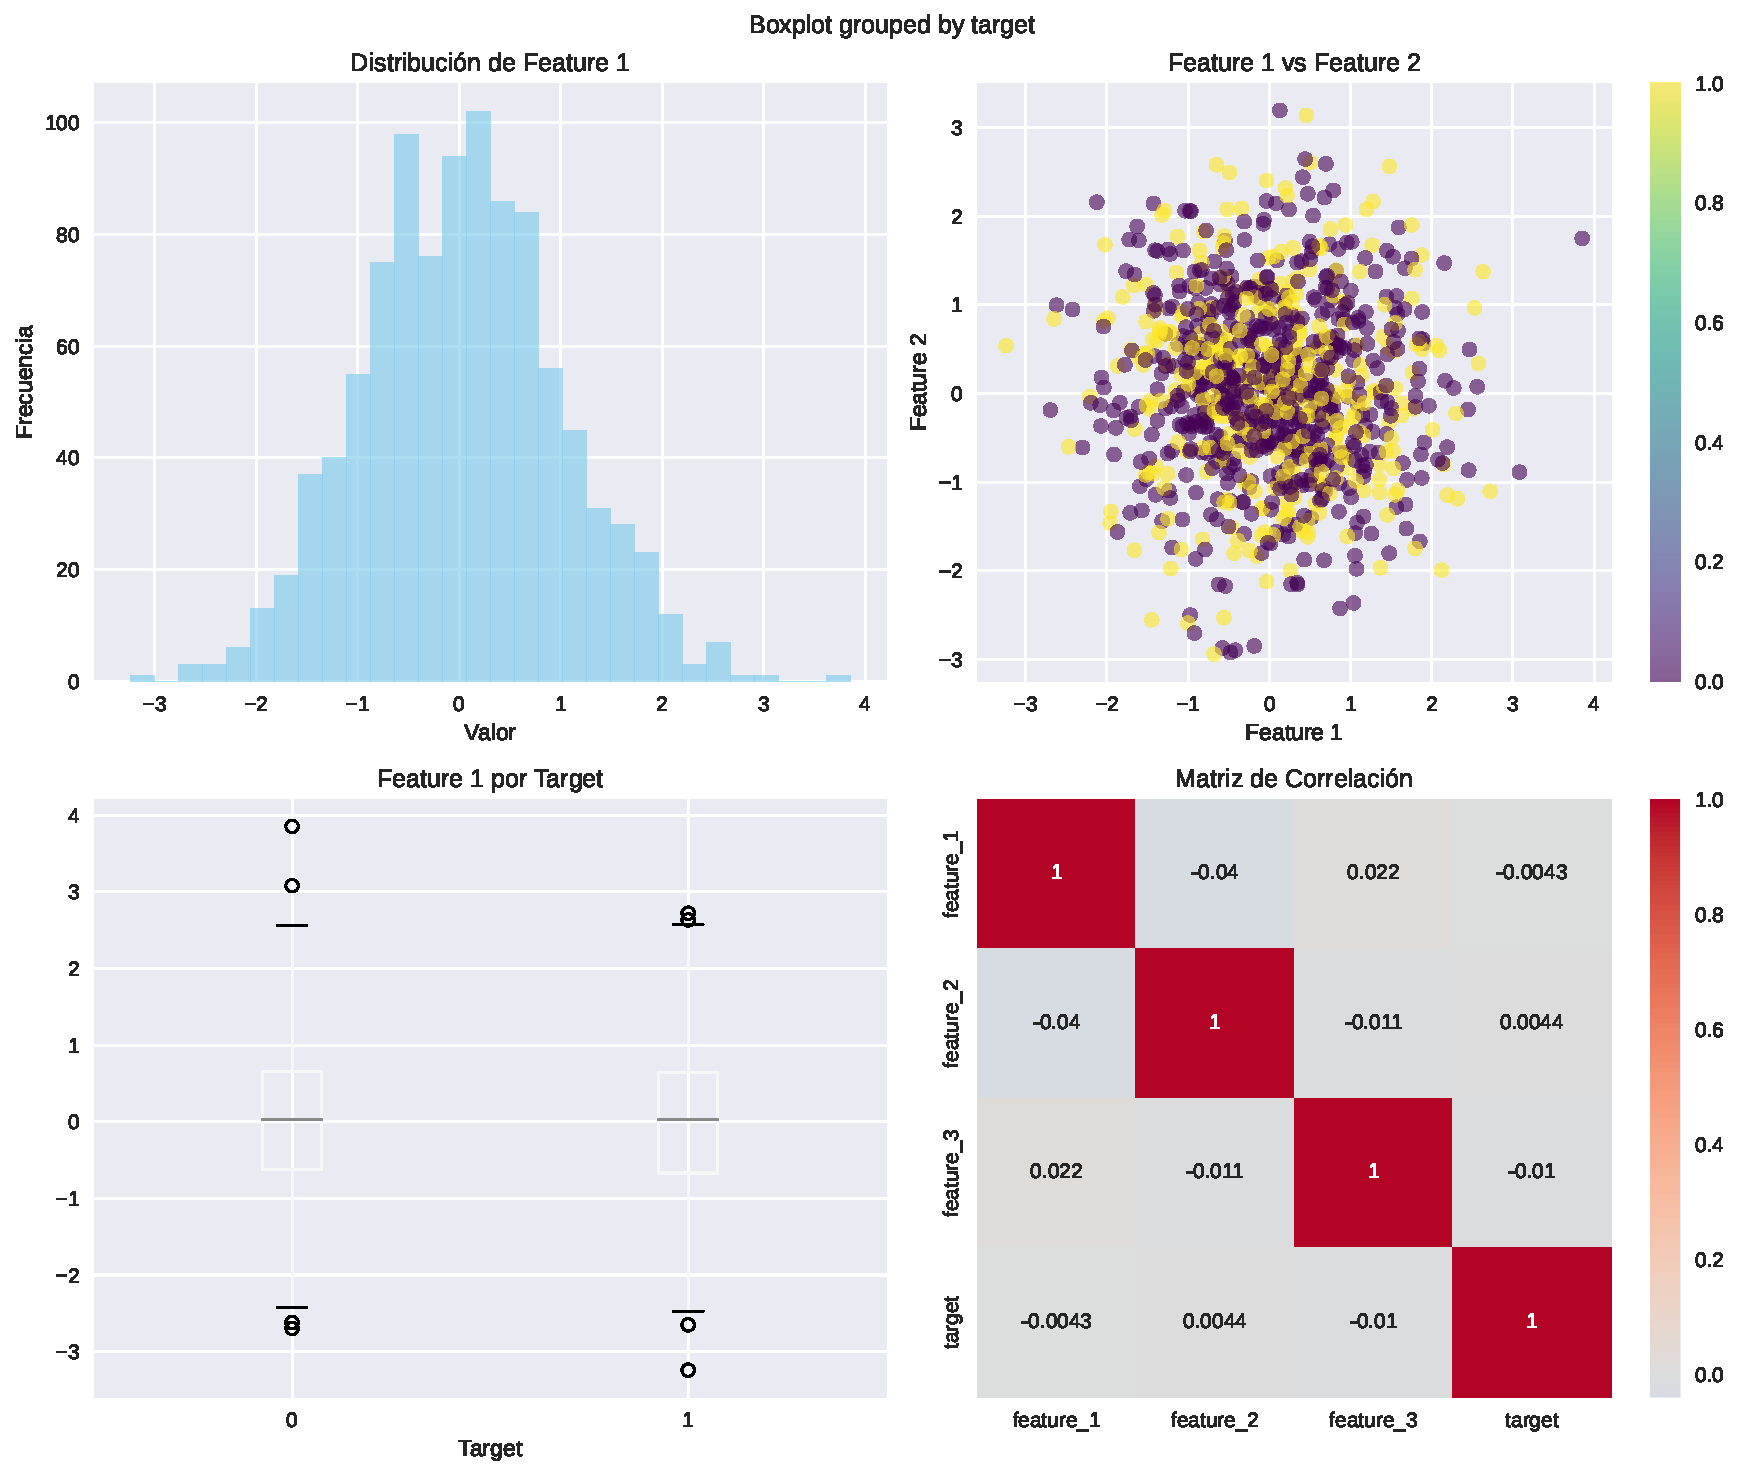
\includegraphics[keepaspectratio]{indexx_files/figure-pdf/visualize-data-output-1.pdf}}

\section{Preparación de Datos}\label{preparaciuxf3n-de-datos}

\phantomsection\label{prepare-data}
\begin{Shaded}
\begin{Highlighting}[]
\CommentTok{\# Separar características y target}
\NormalTok{X }\OperatorTok{=}\NormalTok{ df[[}\StringTok{\textquotesingle{}feature\_1\textquotesingle{}}\NormalTok{, }\StringTok{\textquotesingle{}feature\_2\textquotesingle{}}\NormalTok{, }\StringTok{\textquotesingle{}feature\_3\textquotesingle{}}\NormalTok{]]}
\NormalTok{y }\OperatorTok{=}\NormalTok{ df[}\StringTok{\textquotesingle{}target\textquotesingle{}}\NormalTok{]}

\CommentTok{\# Dividir en conjuntos de entrenamiento y prueba}
\NormalTok{X\_train, X\_test, y\_train, y\_test }\OperatorTok{=}\NormalTok{ train\_test\_split(}
\NormalTok{    X, y, test\_size}\OperatorTok{=}\FloatTok{0.2}\NormalTok{, random\_state}\OperatorTok{=}\DecValTok{42}\NormalTok{, stratify}\OperatorTok{=}\NormalTok{y}
\NormalTok{)}

\BuiltInTok{print}\NormalTok{(}\SpecialStringTok{f"Conjunto de entrenamiento: }\SpecialCharTok{\{}\NormalTok{X\_train}\SpecialCharTok{.}\NormalTok{shape[}\DecValTok{0}\NormalTok{]}\SpecialCharTok{\}}\SpecialStringTok{ muestras"}\NormalTok{)}
\BuiltInTok{print}\NormalTok{(}\SpecialStringTok{f"Conjunto de prueba: }\SpecialCharTok{\{}\NormalTok{X\_test}\SpecialCharTok{.}\NormalTok{shape[}\DecValTok{0}\NormalTok{]}\SpecialCharTok{\}}\SpecialStringTok{ muestras"}\NormalTok{)}
\BuiltInTok{print}\NormalTok{(}\SpecialStringTok{f"Proporción de clases en entrenamiento: }\SpecialCharTok{\{}\NormalTok{y\_train}\SpecialCharTok{.}\NormalTok{value\_counts(normalize}\OperatorTok{=}\VariableTok{True}\NormalTok{)}\SpecialCharTok{\}}\SpecialStringTok{"}\NormalTok{)}
\end{Highlighting}
\end{Shaded}

\begin{verbatim}
Conjunto de entrenamiento: 800 muestras
Conjunto de prueba: 200 muestras
Proporción de clases en entrenamiento: 0    0.62125
1    0.37875
Name: target, dtype: float64
\end{verbatim}

\section{Modelado}\label{modelado}

\subsection{Modelo 1: Regresión
Logística}\label{modelo-1-regresiuxf3n-loguxedstica}

\phantomsection\label{logistic-regression}
\begin{Shaded}
\begin{Highlighting}[]
\CommentTok{\# Entrenar modelo de regresión logística}
\NormalTok{lr\_model }\OperatorTok{=}\NormalTok{ LogisticRegression(random\_state}\OperatorTok{=}\DecValTok{42}\NormalTok{, max\_iter}\OperatorTok{=}\DecValTok{1000}\NormalTok{)}
\NormalTok{lr\_model.fit(X\_train, y\_train)}

\CommentTok{\# Predicciones}
\NormalTok{lr\_pred }\OperatorTok{=}\NormalTok{ lr\_model.predict(X\_test)}
\NormalTok{lr\_pred\_proba }\OperatorTok{=}\NormalTok{ lr\_model.predict\_proba(X\_test)[:, }\DecValTok{1}\NormalTok{]}

\BuiltInTok{print}\NormalTok{(}\StringTok{"Regresión Logística {-} Métricas:"}\NormalTok{)}
\BuiltInTok{print}\NormalTok{(classification\_report(y\_test, lr\_pred))}
\end{Highlighting}
\end{Shaded}

\begin{verbatim}
Regresión Logística - Métricas:
              precision    recall  f1-score   support

           0       0.62      1.00      0.77       124
           1       0.00      0.00      0.00        76

    accuracy                           0.62       200
   macro avg       0.31      0.50      0.38       200
weighted avg       0.38      0.62      0.47       200
\end{verbatim}

\subsection{Modelo 2: Random Forest}\label{modelo-2-random-forest}

\phantomsection\label{random-forest}
\begin{Shaded}
\begin{Highlighting}[]
\CommentTok{\# Entrenar modelo Random Forest}
\NormalTok{rf\_model }\OperatorTok{=}\NormalTok{ RandomForestClassifier(n\_estimators}\OperatorTok{=}\DecValTok{100}\NormalTok{, random\_state}\OperatorTok{=}\DecValTok{42}\NormalTok{)}
\NormalTok{rf\_model.fit(X\_train, y\_train)}

\CommentTok{\# Predicciones}
\NormalTok{rf\_pred }\OperatorTok{=}\NormalTok{ rf\_model.predict(X\_test)}
\NormalTok{rf\_pred\_proba }\OperatorTok{=}\NormalTok{ rf\_model.predict\_proba(X\_test)[:, }\DecValTok{1}\NormalTok{]}

\BuiltInTok{print}\NormalTok{(}\StringTok{"Random Forest {-} Métricas:"}\NormalTok{)}
\BuiltInTok{print}\NormalTok{(classification\_report(y\_test, rf\_pred))}
\end{Highlighting}
\end{Shaded}

\begin{verbatim}
Random Forest - Métricas:
              precision    recall  f1-score   support

           0       0.58      0.72      0.64       124
           1       0.24      0.14      0.18        76

    accuracy                           0.50       200
   macro avg       0.41      0.43      0.41       200
weighted avg       0.45      0.50      0.47       200
\end{verbatim}

\section{Evaluación y Comparación}\label{evaluaciuxf3n-y-comparaciuxf3n}

\subsection{Matriz de Confusión}\label{matriz-de-confusiuxf3n}

\begin{Shaded}
\begin{Highlighting}[]
\NormalTok{fig, axes }\OperatorTok{=}\NormalTok{ plt.subplots(}\DecValTok{1}\NormalTok{, }\DecValTok{2}\NormalTok{, figsize}\OperatorTok{=}\NormalTok{(}\DecValTok{12}\NormalTok{, }\DecValTok{5}\NormalTok{))}

\CommentTok{\# Matriz de confusión para Regresión Logística}
\NormalTok{cm\_lr }\OperatorTok{=}\NormalTok{ confusion\_matrix(y\_test, lr\_pred)}
\NormalTok{sns.heatmap(cm\_lr, annot}\OperatorTok{=}\VariableTok{True}\NormalTok{, fmt}\OperatorTok{=}\StringTok{\textquotesingle{}d\textquotesingle{}}\NormalTok{, cmap}\OperatorTok{=}\StringTok{\textquotesingle{}Blues\textquotesingle{}}\NormalTok{, ax}\OperatorTok{=}\NormalTok{axes[}\DecValTok{0}\NormalTok{])}
\NormalTok{axes[}\DecValTok{0}\NormalTok{].set\_title(}\StringTok{\textquotesingle{}Regresión Logística\textquotesingle{}}\NormalTok{)}
\NormalTok{axes[}\DecValTok{0}\NormalTok{].set\_xlabel(}\StringTok{\textquotesingle{}Predicción\textquotesingle{}}\NormalTok{)}
\NormalTok{axes[}\DecValTok{0}\NormalTok{].set\_ylabel(}\StringTok{\textquotesingle{}Valor Real\textquotesingle{}}\NormalTok{)}

\CommentTok{\# Matriz de confusión para Random Forest}
\NormalTok{cm\_rf }\OperatorTok{=}\NormalTok{ confusion\_matrix(y\_test, rf\_pred)}
\NormalTok{sns.heatmap(cm\_rf, annot}\OperatorTok{=}\VariableTok{True}\NormalTok{, fmt}\OperatorTok{=}\StringTok{\textquotesingle{}d\textquotesingle{}}\NormalTok{, cmap}\OperatorTok{=}\StringTok{\textquotesingle{}Greens\textquotesingle{}}\NormalTok{, ax}\OperatorTok{=}\NormalTok{axes[}\DecValTok{1}\NormalTok{])}
\NormalTok{axes[}\DecValTok{1}\NormalTok{].set\_title(}\StringTok{\textquotesingle{}Random Forest\textquotesingle{}}\NormalTok{)}
\NormalTok{axes[}\DecValTok{1}\NormalTok{].set\_xlabel(}\StringTok{\textquotesingle{}Predicción\textquotesingle{}}\NormalTok{)}
\NormalTok{axes[}\DecValTok{1}\NormalTok{].set\_ylabel(}\StringTok{\textquotesingle{}Valor Real\textquotesingle{}}\NormalTok{)}

\NormalTok{plt.tight\_layout()}
\NormalTok{plt.show()}
\end{Highlighting}
\end{Shaded}

\pandocbounded{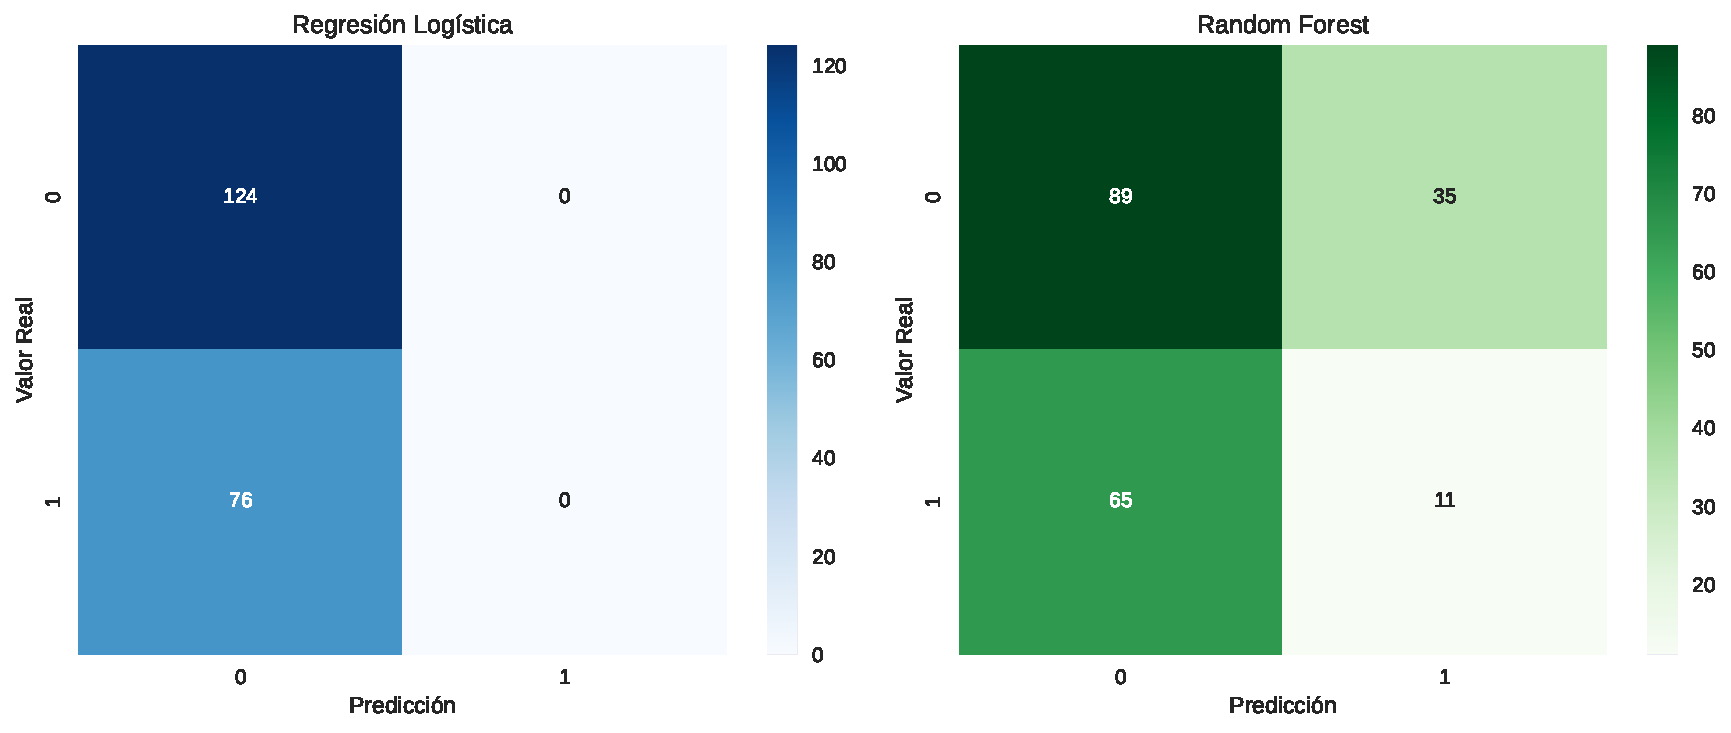
\includegraphics[keepaspectratio]{indexx_files/figure-pdf/confusion-matrices-output-1.pdf}}

\subsection{Comparación de Importancia de
Características}\label{comparaciuxf3n-de-importancia-de-caracteruxedsticas}

\begin{Shaded}
\begin{Highlighting}[]
\CommentTok{\# Importancia de características para Random Forest}
\NormalTok{feature\_importance }\OperatorTok{=}\NormalTok{ pd.DataFrame(\{}
    \StringTok{\textquotesingle{}feature\textquotesingle{}}\NormalTok{: X.columns,}
    \StringTok{\textquotesingle{}importance\textquotesingle{}}\NormalTok{: rf\_model.feature\_importances\_}
\NormalTok{\}).sort\_values(}\StringTok{\textquotesingle{}importance\textquotesingle{}}\NormalTok{, ascending}\OperatorTok{=}\VariableTok{True}\NormalTok{)}

\NormalTok{plt.figure(figsize}\OperatorTok{=}\NormalTok{(}\DecValTok{10}\NormalTok{, }\DecValTok{6}\NormalTok{))}
\NormalTok{plt.barh(feature\_importance[}\StringTok{\textquotesingle{}feature\textquotesingle{}}\NormalTok{], feature\_importance[}\StringTok{\textquotesingle{}importance\textquotesingle{}}\NormalTok{])}
\NormalTok{plt.title(}\StringTok{\textquotesingle{}Importancia de Características {-} Random Forest\textquotesingle{}}\NormalTok{)}
\NormalTok{plt.xlabel(}\StringTok{\textquotesingle{}Importancia\textquotesingle{}}\NormalTok{)}
\NormalTok{plt.tight\_layout()}
\NormalTok{plt.show()}
\end{Highlighting}
\end{Shaded}

\pandocbounded{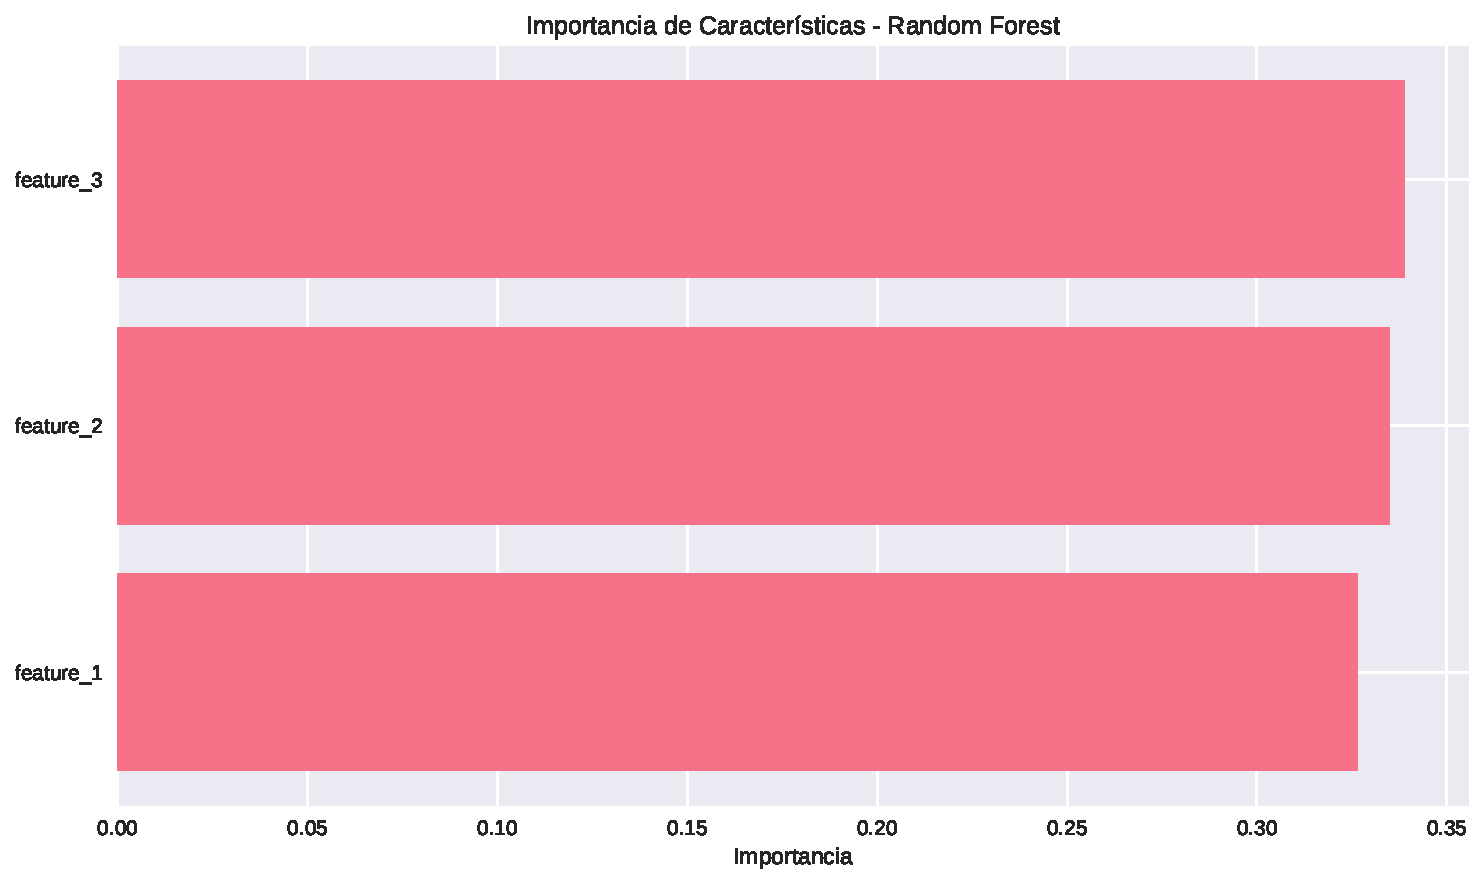
\includegraphics[keepaspectratio]{indexx_files/figure-pdf/feature-importance-output-1.pdf}}

\section{Resultados y Conclusiones}\label{resultados-y-conclusiones}

\subsection{Resumen de Resultados}\label{resumen-de-resultados}

Los modelos implementados muestran diferentes niveles de rendimiento:

\begin{itemize}
\tightlist
\item
  \textbf{Regresión Logística}: Modelo lineal simple y rápido
\item
  \textbf{Random Forest}: Modelo más complejo con mejor capacidad de
  capturar relaciones no lineales
\end{itemize}

\subsection{Próximos Pasos}\label{pruxf3ximos-pasos}

\begin{enumerate}
\def\labelenumi{\arabic{enumi}.}
\tightlist
\item
  Probar otros algoritmos (SVM, XGBoost, etc.)
\item
  Optimizar hiperparámetros
\item
  Implementar validación cruzada
\item
  Análisis de más características
\end{enumerate}

\begin{center}\rule{0.5\linewidth}{0.5pt}\end{center}

\emph{Documento generado con Quarto - \{format(Sys.time(), ``\%Y-\%m-\%d
\%H:\%M:\%S'')\}}




\end{document}
